\capitulo{5}{Resultados}
Los resultados obtenidos en este Trabajo de Fin de Grado muestran la viabilidad de desarrollar una herramienta capaz de integrar información farmacológica procedente de distintas bases de datos heterogéneas con el objetivo de detectar posibles interacciones entre principios activos.

\section{Funcionamiento de la interfaz}
En relación con el objetivo general, se ha logrado implementar un sistema funcional que permite analizar la interacción entre fármacos a partir de las enzimas implicadas en su metabolismo. La herramienta desarrollada proporciona una visualización clara de los resultados, facilitando de esta manera la interpretación por parte del usuario final.

Todos los ejemplos mostrados en los siguientes resultados son para la interacción clopidogrel-omeprazole. Además, todas las explicaciones se encuentran en inglés debido a que, de esta manera, la aplicación podrá ser utilizada por cualquier persona.

Una vez dentro de la plataforma se encuentra la interfaz principal \ref{fig:pag_ppal} que posee un logo creado en la parte superior, una breve descripción de la funcionalidad de la herramienta y las enzimas tenidas en cuenta para la interacción junto a un menú lateral con las diferentes pestañas en las que introduciremos cada uno de los principios activos. 
\begin{figure}[h]
    \centering
    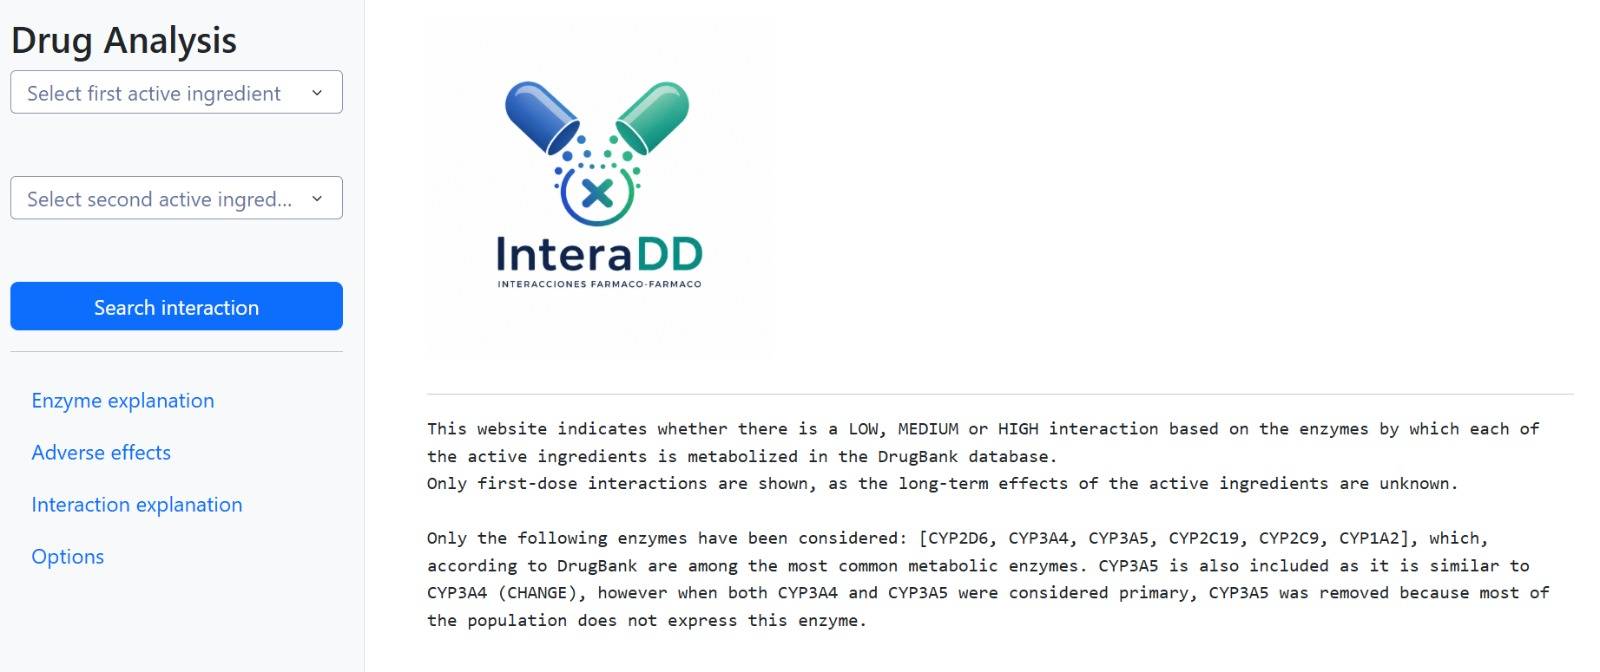
\includegraphics[width=0.5\textwidth]{img/pagina_principal.jpeg} 
    \caption{Página principal de la herramienta desarrollada}
    \label{fig:pag_ppal}
\end{figure}

Tras introducir los pares de principios activios y pulsar el boton de “search interaction” nos aparece el nivel de interacción en un cuadro de texto codificado por colores (rojo/amarillo/verde) y en caso necesario de saber el porque de dicho nivel, hay un desplegablee con la correspondiente explicación visible en la siguiente imagen \ref{fig:buscar_interaccion}. Esta información nunca se elimina de la interfaz visual hasta el momento en el que se busca otra interacción diferente con otros principios activos distintos. 

\begin{figure}[h]
    \centering
    
\includegraphics[width=0.5\textwidth]{img/interaccion.jpeg} 
    \caption{Cuadro fijo}
    \label{fig:buscar_interaccion}
\end{figure}

Por otro lado, el botón "enzyme explanation" nos ofrece las enzimas principales de los principios activos solicitados, en caso de tenerlas, y una breve explicación del criterio de selección de dichas enzimas, un ejemplo del mismo es el visto en la siguiente imagen \ref{fig:enzimas}.

\begin{figure}[h]
    \centering
    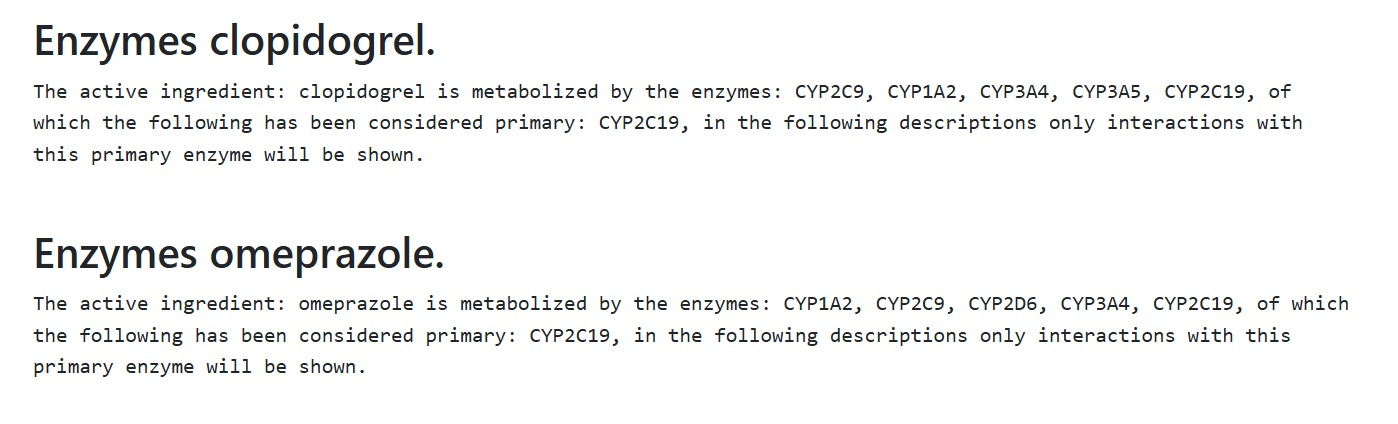
\includegraphics[width=0.5\textwidth]{img/exp_enz.jpeg} 
    \caption{Explicación de enzimas}
    \label{fig:enzimas}
\end{figure}

En el módulo de efectos adversos, nos muestra en un gráfico de barras interactivo, los principales efectos adversos según el/los código/s ATC de referencia de cada principio activo introducido, se puede ver en la imagen adjunta \ref{fig:grafico_ea}.

\begin{figure}[h]
    \centering
    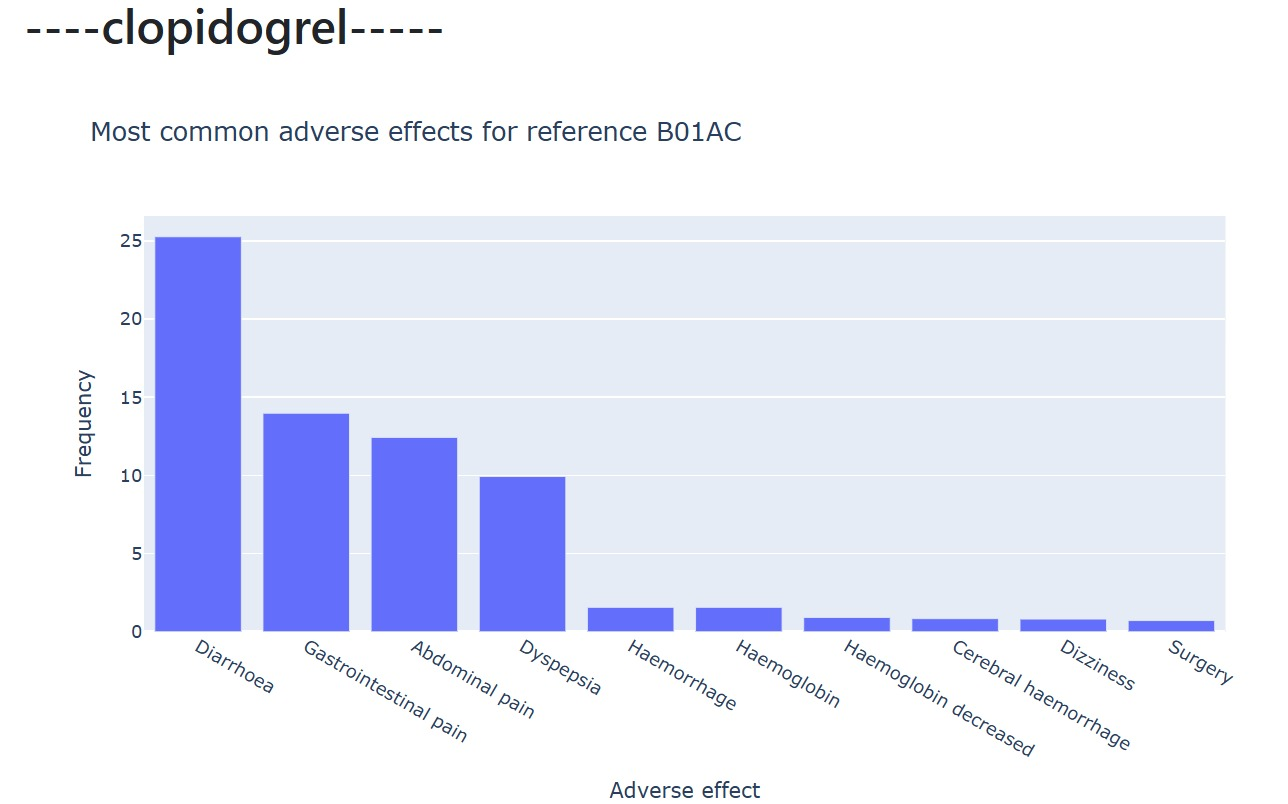
\includegraphics[width=0.5\textwidth]{img/diagrama_ea.jpeg} 
    \caption{Diagrama de barras de efectos adversos}
    \label{fig:grafico_ea}
\end{figure}

Otro de los botones incluidos "Interaction explanation" explica el mecanismo de acción que siguen ambos principios para las enzimas detectadas por el algoritmo como coincidentes, indicando de esta manera el nivel de prevalencia de una sobre otra, se puede observar en la siguiente imagen \ref{fig:acciones}.

\begin{figure}[h]
    \centering
    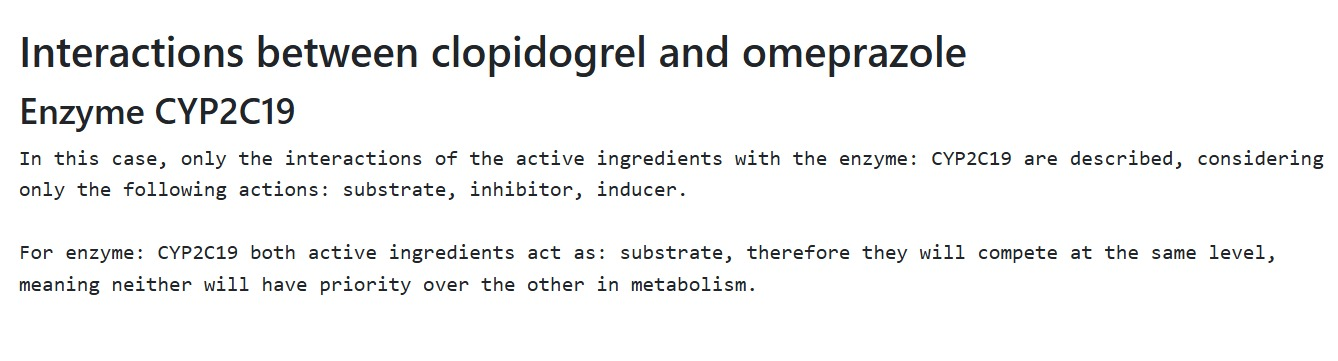
\includegraphics[width=0.5\textwidth]{img/exp_acciones.jpeg} 
    \caption{Explicación de las acciones de cada enzima que hace que los principios interactúen.}
    \label{fig:acciones}
\end{figure}

Finalmente, en la pestaña "options" podemos ver alternativas terapéuticas consideradas seguras para el algoritmo, en caso de que la interacción entre los principios activos resulte ser media-alta, se muestran las alternativas para los principios activos seleccionados en la imagen \ref{fig:alternativas}.

\begin{figure}[h]
    \centering
    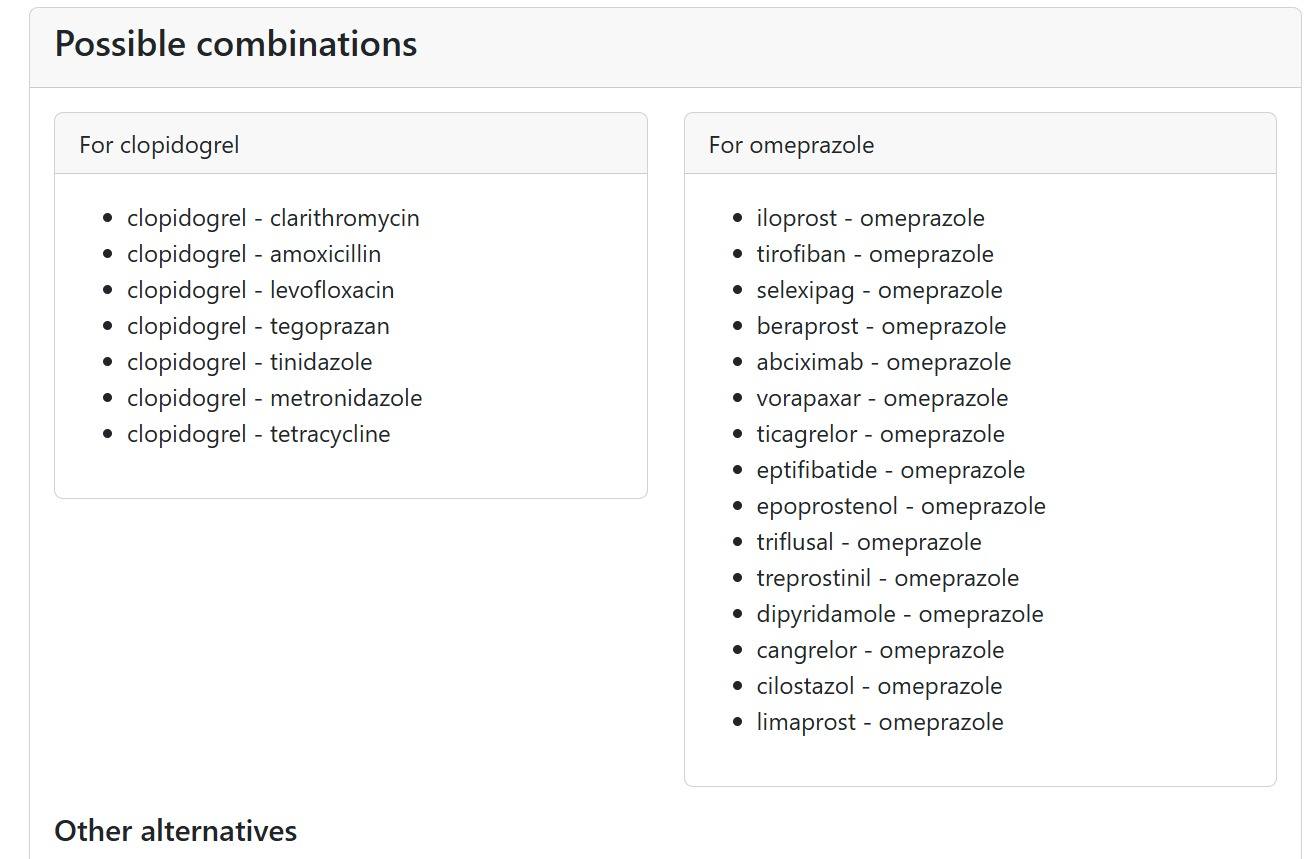
\includegraphics[width=0.5\textwidth]{img/opciones.jpeg} 
    \caption{Posibles alternativas terapéuticas clopidogrel-omeprazole.}
    \label{fig:alternativas}
\end{figure}

En conjunto, el sistema desarrollado cumple los objetivos planteados, proporcionando una herramienta funcional para el análisis de interacciones farmacológicas y proposición de alternativas seguras. No obstante, su uso debe entenderse como un sistema de apoyo a la decisión y no como una herramienta clínica definitiva.

\section{Casos de prueba}

PRIMERO TENGO QUE SOLUCIONAR EL RENDER